\addtorecentlist{Overleaf}
    
\begin{frame}
    \frametitle{Overleaf}

    %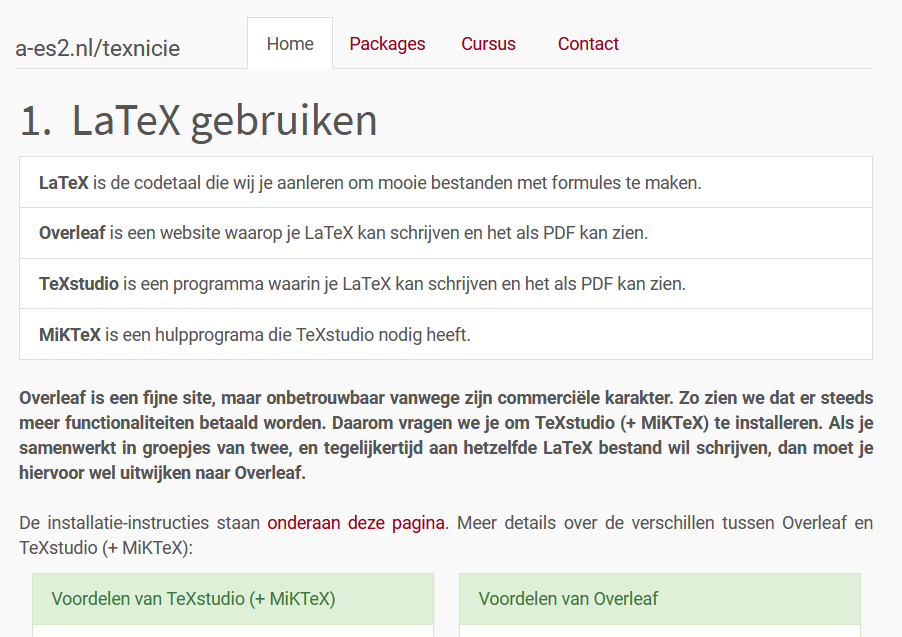
\includegraphics[trim=10px 120px 50px 30px,clip,width=0.95\textwidth]{texnicieWebsiteOverleafTeXstudio.png}
    \lang{
        \begin{list}{}{
            \itemindent-\leftmargin
            \setlength{\itemsep}{2pt}
        }
            \item\textbf{LaTeX} is the programming language.
            \item\textbf{Overleaf} is a website where you can write and
                compile LaTeX.
            \item\textbf{Visual Studio Code} is a desktop app where you can
                write and compile LaTeX.
            \item\textbf{MiKTeX} does compilation for Visual Studio code.
        \end{list}
    }{
        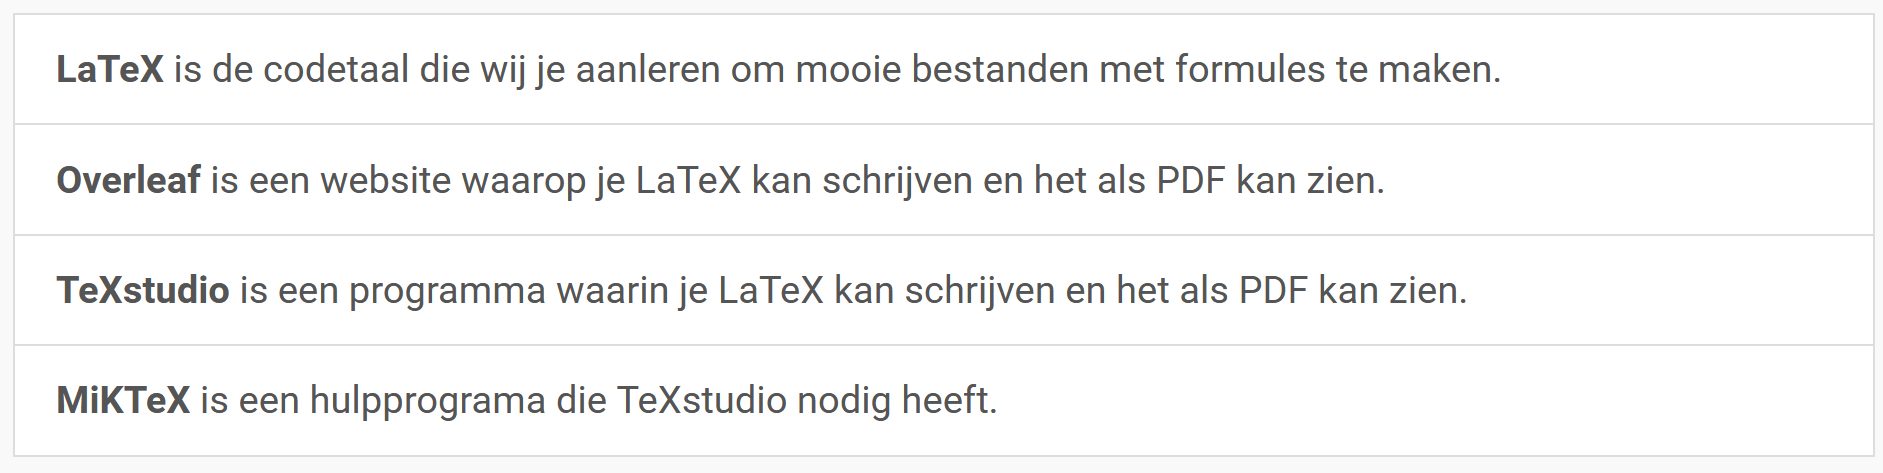
\includegraphics[width=\textwidth]{\assetdir/overleafDisambiguation.png}
    }

    \begin{columns}
        \begin{column}{0.3\textwidth}
            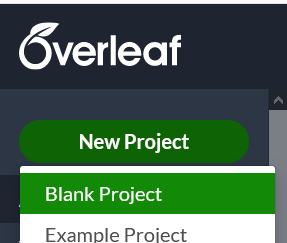
\includegraphics[width=\linewidth]{\assetdir/overleafCreateBlankProject.png}
        \end{column}
        \begin{column}{0.7\textwidth}
            \lang{%
                For now: Overleaf.
            }{%
                %Op het einde nog woordje hierover.
                
                Voor nu: Overleaf.
            }
            
            \medskip
            \lang{%
                Want VS Code? Instructions at
                \href{https://vkuhlmann.com/latex/installation}{\nolinkurl{vkuhlmann.com/latex/installation}}
            }{%
                Nu al niet-commerci\"ele variant installeren? \url{a-es2.nl/texnicie}
            }
        \end{column}
    \end{columns}
\end{frame}
